
%%% Local Variables: 
%%% mode: latex
%%% TeX-master: "../notes"
%%% End: 


\def\w{2}
\def\h{1.5}
\def\xdelta{1.5}
\def\ydelta{1}
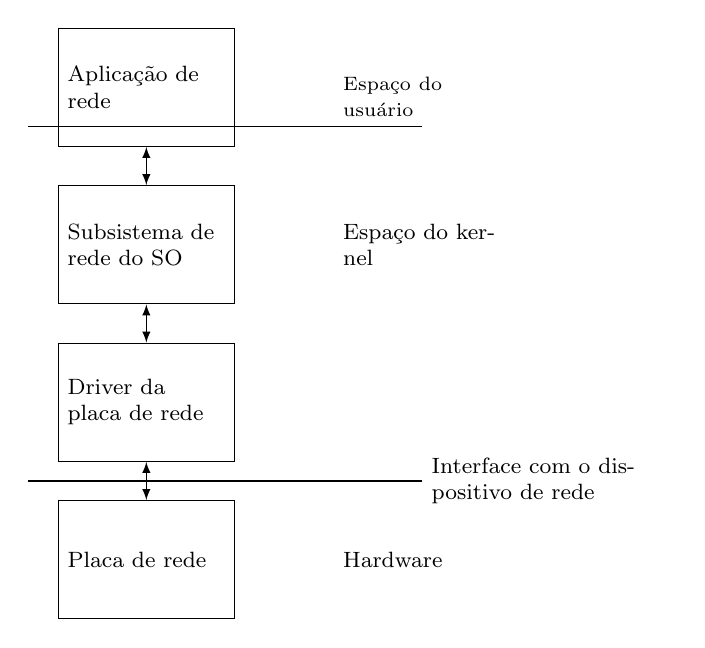
\begin{tikzpicture}
  \tikzset{every node/.style={text width=2cm,font={\footnotesize}},
  module/.style={rectangle,minimum height=1.5cm,draw}}
  \foreach \y/\l in {0/{Aplicação de rede},-2/{Subsistema de rede do
      SO},-4/{Driver da placa de rede},-6/{Placa de rede}} {
    \node[module] (\y) at (0,\y+\h) {\l};
  }
  \foreach \s/\d in {0/-2,-2/-4,-4/-6} {
    \path[<->,>=latex,draw] (\s) -- (\d);
  }

  \draw (-\xdelta,\ydelta) -- (\w+\xdelta,\ydelta) node[above]
  {\scriptsize Espaço
  do usuário};
\node [right of=-2,xshift=25mm] {Espaço do kernel};

  \draw (-\xdelta,-3.5) -- (\w+\xdelta,-3.5) node[text width=3cm,right] {Interface com o
    dispositivo de rede};
  \node [right of=-6,xshift=25mm] {Hardware};
\end{tikzpicture}